\tikzset{
   plane/.pic = {
    \draw[fill]  plot[smooth, tension=0.6] coordinates {
        (-0.65,-0.9) 
        (-0.6,-0.85) 
        (-0.4,-0.75) 
        (-0.25,-0.65) 
        (-0.15,-0.5) 
        (-0.12,-0.3) 
        (-0.1,-0.1) 
        (0,0) 
        (0.1,-0.1) 
        (0.12,-0.3) 
        (0.15,-0.5) 
        (0.25,-0.65) 
        (0.4,-0.75) 
        (0.6,-0.85) 
        (0.65,-0.9)
        } -- plot[smooth, tension=0.6] coordinates {
        (0.65,-0.9) 
        (0.15,-0.91)
        (0.35,-1.1) 
        (0.37,-1.15)
        } -- plot[smooth, tension=0.6] coordinates {
        (0.37,-1.15)
        (0,-1.12) 
        (-0.37,-1.15) 
        } -- plot[smooth, tension=0.6] coordinates {
        (-0.37,-1.15)
        (-0.35,-1.1) 
        (-0.15,-0.91) 
        (-0.65,-0.9) 
        } -- cycle;
   }
}
\newcommand{\rvec}[1]{\ensuremath{{\boldsymbol{\underline{#1}}}}}
\newcommand{\rv}[1]{\ensuremath{{\boldsymbol{#1}}}}
\newcommand{\mat}[1]{{\ensuremath{{\mathbf{#1}}}}}

\usetikzlibrary{math}

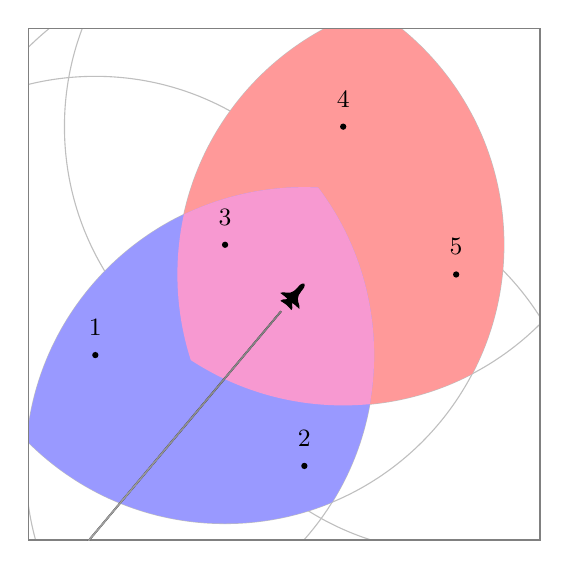
\begin{tikzpicture}[font=\small]
    % Sizes
    \tikzmath{\srange = 3.54; \sradius = 0.04;}
    % Sensor locations (sensor 3 is shared)
    \coordinate (s1) at (0.8523,-4.1508) {};
    \coordinate (s2) at (3.507,-5.5587) {};
    \coordinate (s3) at (2.5,-2.75) {} {};
    \coordinate (s4) at (4,-1.25) {};
    \coordinate (s5) at (5.4346,-3.1274) {};
    % Navigator location
    \coordinate (nav_loc) at (3.5,-3.25) {};
    % Bounding rectangle
    \coordinate (brect_start) at (0,0);
    \coordinate (brect_end) at (6.5, -6.5);
    
    % Gray range circles
    \begin{scope}
        \clip (brect_start) rectangle (brect_end);
        \draw[gray!50] (s1) circle (\srange);
        \draw[gray!50] (s2) circle (\srange);
        \draw[gray!50] (s3) circle (\srange);
        \draw[gray!50] (s4) circle (\srange);
        \draw[gray!50] (s5) circle (\srange);
    \end{scope}
    % Red subgroup overlap
    \begin{scope}
        \clip (brect_start) rectangle (brect_end);
        \clip (s3) circle (\srange);
        \clip (s4) circle (\srange);
        \clip (s5) circle (\srange);
        \fill[red!40] (brect_start) rectangle (brect_end);
    \end{scope}
    % Blue subgroup overlap
    \begin{scope}
        \clip (brect_start) rectangle (brect_end);
        \clip (s1) circle (\srange);
        \clip (s2) circle (\srange);
        \clip (s3) circle (\srange);
        \fill[blue!40] (brect_start) rectangle (brect_end);
    \end{scope}
    % Magenta double overlap
    \begin{scope}
        \clip (brect_start) rectangle (brect_end);
        \clip (s1) circle (\srange);
        \clip (s2) circle (\srange);
        \clip (s3) circle (\srange);
        \clip (s4) circle (\srange);
        \clip (s5) circle (\srange);
        \fill[magenta!40] (brect_start) rectangle (brect_end);
    \end{scope}
    % Sensors
    \fill[black] (s1) circle (\sradius);
    \fill[black] (s2) circle (\sradius);
    \fill[black] (s3) circle (\sradius);
    \fill[black] (s4) circle (\sradius);
    \fill[black] (s5) circle (\sradius);
    % Bounding box
    \draw[gray] (brect_start) rectangle (brect_end);
    % Navigator
    \clip (brect_start) rectangle (brect_end);
    \pic[rotate=-40,xscale=0.22,yscale=0.3] at (nav_loc) {plane};
    \begin{scope}[shift={(nav_loc)},rotate=-40,xscale=0.22,yscale=0.3]
        % Trail
        \fill[bottom color=white, top color=gray] (-0.05, -1.5) rectangle (0.05, -50);
    \end{scope}
    % Sensor labels
    \node[label=1] at (s1) {};
    \node[label=2] at (s2) {};
    \node[label=3] at (s3) {};
    \node[label=4] at (s4) {};
    \node[label=5] at (s5) {};
\end{tikzpicture}













